In the previous section, we showed some limitations of the EFC permission structure and token-based reasoning. However, those limitations could be overcome, though they made proofs less intuitive and hence harder to write. In this section, we will develop on some limitations of FSL++. Those limitations seem more fundamental, as we could not find ways to overcome them, and at least one would require an extension to the FSL++ logic. We will develop those limitations using two examples, from the glibc and Folly libraries.

\section{glibc Reader-Writer Lock}
We will first focus on the glibc Reader-Writer lock \cite{glibcRW}. As we will see in Section~\ref{subsec:glibcRWPb}, it cannot be proven in FSL++ for a deceptively simple reason. We will still describe it in details, as its synchronization mechanism is quite interesting, and shows how a slightly different implementation can make for different (or impossible in this case) proofs.

\subsection{Implementation}
The implementation of this lock is shown in Appendix~\ref{app:glibc}. This implementation was heavily simplified from the original one.% In particular, futexes (special variables used to wake-up a thread when an event occurs) which where used to prevent extra spining where removed. While they are important to make the code more efficient, they are not part of the synchronization mechanisms used to ensure correctness of this lock.

\begin{figure}
		\begin{center}
		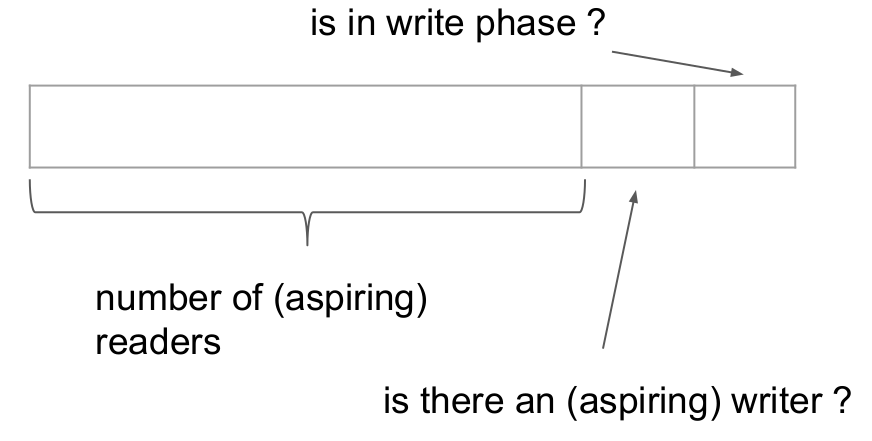
\includegraphics[width=\linewidth]{schemaglibc.png}
		%\caption{glibc reader-writer lock}
		\end{center}
		\caption{glibc reader-writer lock}
		\label{schemaglibc}
\end{figure}

Just as the Folly reader-writer lock, this lock offers four main functions: \texttt{readLock} (equivalent of \texttt{lock\_shared}), \texttt{readUnlock} (\texttt{unlock\_shared}), \texttt{writeLock} (\texttt{lock}) and \texttt{writeUnlock} (\texttt{unlock}).

This implementation uses a single atomic location \texttt{\_\_readers}, used similarly as the location \texttt{bits} in the Folly reader writer lock. This location is used as shown in Figure~\ref{schemaglibc}. The least significant bit is used to denote if the lock is in read or write phase. As can be expected, if it is in read phase, only reader access can be granted, while if it is in write phase, only writer access can be granted. The second least significant bit tells whether or not there is currently a thread asking for or having write access. Finally, \texttt{\_\_readers} $/ 8$ gives us the number of threads currently owning reader access or requesting it. For easier reading, we use the following denotation for the value of \texttt{readers\_\_}: $\mathtt{readers\_\_} / 8 | lsb(\mathtt{readers\_\_ }/ 2) | lsb(\mathtt{readers\_\_})$. For instance, $2|1|1$ corresponds to \texttt{readers\_\_} $=19$, which means the lock is currently in write phase, and that one thread owns a write access, while two threads are requesting a read access. If it were to contain $2 | 0 | 1$, it means it is still in write mode, but no thread owns write access to it. The implementation makes sure that in this case one of the threads requesting read access will change the least significant bit to $0$, allowing for read access.

Each of the functions then uses appropriate synchronization mechanisms to ensure the value of \texttt{\_\_readers} accurately reflects the permissions threads hold to the protected location, as well as proper synchronization when taking or releasing the lock. A more detailed explanation of the lock implementation can be found in the Appendix~\ref{app:glibc}. The synchronization mechanisms are quite complex, and not necessary to understand the following.

We will here only focus on a further simplification of the \texttt{readerLock} function which is sufficient to show the different mechanisms we are interested in. 
%We simply remove loops and replace them with \texttt{if} statements. Note that note only the call to lock can now fail, but it may also put the lock in an inconsistent state (as it may increment the number of readers, and never decrement it). However, we are here only interested in successfull executions of this simplification. 
This simple code is shown in Figure~\ref{fig:codeglibc}.

\begin{figure}
		\begin{lstlisting}
Constants:
WRLOCKED = 2
WRPHASE = 1

int readLock(){
	int r = fetchAndAdd_Acq(__readers, 8) + 8
	if(r & WRPHASE == 0)
		return 0
	while(r & WRPHASE != 0 && r & WRLOCKED == 0){...}

	while(Load_Acq(__readers) & WRPHASE == 1){;}
}

	\end{lstlisting}
	\caption{\texttt{readLock function}}
	\label{fig:codeglibc}
\end{figure}
In the rest of this section, we will only use two executions scenarios to support our reasoning. They are shown in Figure~\ref{fig:scen1} and Figure~\ref{fig:scen2}. The first one is the most straightforward: there is only one thread trying to get the lock. It calls \texttt{readLock()}. The \texttt{fetchAndAdd} occurs, increasing the number of potential reader threads by 1. We then check if the least significant bit (corresponding to \texttt{WRITEPHASE}) is set to 0. As it is the case, the function returns: Thread 1 now has a read lock. In the second scenario, Thread 1 holds a write lock when Thread 2 calls the \texttt{readLock} function. Hence after the \texttt{fetchAndAdd}, neither the \texttt{if} condition nor the following \texttt{while} condition succeed. Thread 1 then releases the lock. The condition of the final \texttt{while} is then satisfied. The function returns and Thread 2 now holds a read lock.

We see here that the calling thread can get read access to the resource in two distinct points \footnote{There is actually a third one in the elided code, but it is not relevant to our discussion here}. This is quite different from the Folly reader-writer spinlock implementation, where the access was granted by the \texttt{fetchAndAdd} operation only. If the lock was already taken, the function would cancel this add (by subtracting the same value), and fail. We will see now how this proves to be a problem when formalizing this lock in FSL++.


\begin{figure}
\begin{tabular}{c||c}
	\texttt{\_\_readers} & Thread 1\\
	0 | 0 | 0 & \\
	 &   \texttt{fetchAndAdd\_(\_\_readers)} \\
	1 | 0 | 0 & \\
	 & \texttt{if(r \& WRPHASE == 0) } \\
	& \texttt{return 0 } \\
	&  Read lock succeeds!
\end{tabular}

		\caption{First \texttt{readLock()} execution scenario}
		\label{fig:scen1}
		%\caption{First \texttt{readLock()} execution scenario}
\end{figure}
\begin{figure}
\begin{tabular}{c||c|c}
	\texttt{\_\_readers} & Thread 1 & Thread 2 \\
	0 | 0 | 0 & & \\
	 & \texttt{writeLock()} & \\
	0 | 1 | 1 &   & \\
	 &   & \texttt{fetchAndAdd\_(\_\_readers)} \\
	1 | 1 | 1 & & \\
		& & \texttt{if(r \& WRPHASE == 0) ...} \\
		& & \texttt{while(r \& WRPHASE != 0 ...} \\
	 & \texttt{writeUnlock()} & \\
		1 | 0 | 0 & & \\
		& & \texttt{Load\_Acq(\_\_readers) \& WRPHASE} \\
		& & Read lock succeeds!
\end{tabular}

		\caption{Second \texttt{readLock()} execution scenario}
		\label{fig:scen2}
		%\caption{Second \texttt{readLock()} execution scenario}
\end{figure}


		\subsection{Read-Modify-Write and Load}
	\label{subsec:glibcRWPb}
As we saw in the two executions scenarios described above, read permission can be given either by a fetch-and-add, or by a subsequent load. However, when looking into the proof rules of FSL++, none of them allow for gaining resources from a single atomic location both using a Load and a fetch-and-add. When looking further into it becomes quite clear why such a rule would be quite difficult to implement.

In FSL++, atomic locations are used to transfer ownership (here to the resources protected by the lock) between threads. It does so by using a location invariant $\mathcal{Q}$ which for each value $v$ gives the ownership corresponding to this value. Then when writing value $v$ to the atomic location, a thread has to give up the assertion $\mathcal{Q}(v)$, and when reading value $v$, a thread gains this assertion. However this simplistic idea is not sufficient: it could happen that Thread 1 writes $v$, giving up $\mathcal{Q}(v)$, then Thread 2, reads $v$, gaining $\mathcal{Q}(v)$, then Thread 3 reads as well $v$, gaining $\mathcal{Q}(v)$. Here, the assertion $\mathcal{Q}(v)$ has been duplicated, which is clearly unsound \footnote{For instance if $\mathcal{Q}(v) = \ress{1}$, this would lead to total permission access to a location striclty greater than 1.}. To forbid this outcome, FSL++ introduces the assertions $\acqPerm$ and $\relPerm$. When a new variable is created, the corresponding permissions $\{\acqPerm * \relPerm\}$ are created. $\relPerm$ can then be freely duplicated, whereas the $\acqPerm$ can only be transmitted, making sure only one thread is allowed to get ownership from the location (all threads can read from the location, but they will get no ownership from it). 

Now for read-modify-write operations, that is to say operations that read and write atomically to a variable, the situation is different. As the value of the variable is read and changed in one atomic operation, the duplicating problem does not occur anymore. If thread 1 does a fetch-and-add and reads value $v$, it gets $\mathcal{Q}(v)$, and gives $\mathcal{Q}(v + 1)$. Hence if another thread then does another fetch-and-add there is no risk of inadvertently getting twice the same permission. Hence we can be more permissive here, allowing multiple threads to perform read-modify-writes to the same location, and all gaining ownership. To allow for this, when a new variable is created, FSL++ offers a choice between $\relPerm * \acqPerm$ or $\relPerm * \rmwPerm$. The latter is then freely duplicable and can be transmitted to all threads requiring it. There is however no rule that would allow to have both $\operatorname{\mathsf{Acq}}(\ell, \mathcal{Q}_1)$and $\operatorname{\mathsf{RMWAcq}}(\ell, \mathcal{Q}_2)$ for the same location, with $\mathcal{Q}_1$ not empty.

A new logic rule that would allow for this would be difficult to design, as it would have to take into account the duplicability of $\rmwPerm$ and non duplicability of $\acqPerm$.

	\subsection{Separation of tokens and permission}
We saw in the previous section how FSL++ rules do not allow for a proof of the glibc reader-writer lock. Another interesting point of this lock when thinking in terms of the EFC permission structure, is that it separates tokens from permission. In the second scenario Figure~\ref{fig:scen2}, thread 2 increments the number of readers with the fetch-and-add, but only gets permission with the load in the second while. This would hence make counting the number of permissions given away (as recorded by \texttt{\_\_readers / 8}) difficult to link with the amount of permission given (done in the load here).
